\documentclass{school-22.101-notes}
\date{September 26, 2011}

\begin{document}
\maketitle




%%%%%%%%%%%%%%%%%%%%%%%% Tunneling %%%%%%%%%%%%%
\topic{Rectangular Barrier \& Tunneling} \label{rectangular-barrier}
$x<0$ is region 1, $x=0$ to $x=L$ is region 2 with a potential barrier of $V_H$, and $x>L$ is region 3. Case A: incoming energy $E > V_H$. Case B: $E < V_H$. 

\subtopic{Case A: $E > V$}
\begin{itemize}
\begin{figure}[ht]
    \centering
    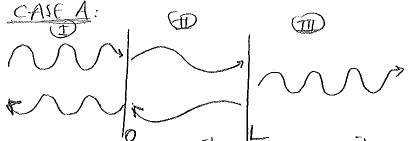
\includegraphics[width=4in]{images/qm/rectangular-caseA.png}
    \caption{Rectangular Barrier Diagram, E$>$V}
    \label{rectangular-caseA}
\end{figure}
\item We write expression for the three regions (the right-most region should never have particles travelling to the left): 
\eqn{ \psi_1 (x) = A e^{ik_1 x} + B e^{-ik_1 x}, \psi_2 (x) = C e^{ik_2 x} + D e^{-ik_2 x}, \psi_3 (x) = E e^{ik_1 x} }
where $k_1 =  \sqrt{\frac{2 m E_1}{\hbar^2}}, k_2 = \sqrt{\frac{2 m (E_1 - V_H)}{\hbar^2}}$. See Figure~\ref{rectangular-caseA}.


\item Notice the transmitted wave is the one in Region 3. We can write: 
\eqn{ \left.  \begin{array}{c} T = \frac{\frac{\hbar k_1}{m} |E|^2}{\frac{\hbar k_1}{m} |A|^2} = \frac{|E|^2}{|A|^2}  \\ R = \frac{\frac{\hbar k_1}{m} |B|^2}{\frac{\hbar k_1}{m} |A|^2} = \frac{|B|^2}{|A|^2}   \end{array} \right\} 1  = T+R  }

\item BCs: $\psi(x)$ is continuous, $\dpsidx$ is continuous, so $\frac{1}{\psi (x)} \dpsidx$ is continuous. This latter expression is often times easier mathematically for solving the BCs. 

\end{itemize}

\subtopic{Case B: $E < V$}
\begin{itemize}
\begin{figure}[ht]
    \centering
    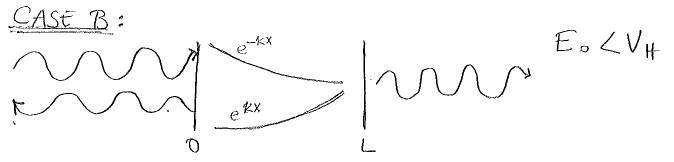
\includegraphics[width=3.5in]{images/qm/rectangular-caseB.png}
    \caption{Rectangular Barrier Diagram, E$<$V}
\end{figure}

\item We write expression for the three regions: 
\eqn{ \psi_1 (x) = A e^{ik_1 x} + B e^{-ik_1 x}, \psi_2 (x) = C e^{\kappa x} + D e^{-\kappa x}, \psi_3 (x) = E e^{ik_1 x} }
in which $k_1 =  \sqrt{\frac{2 m E_1}{\hbar^2}}, k_2 = \sqrt{\frac{2 m (E_1 - V_H)}{\hbar^2}}, \kappa^2 = - k_2^2, \kappa = i k_2$. 

\begin{figure}[ht]
    \centering
    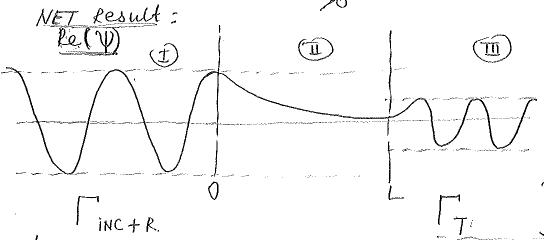
\includegraphics[width=4in]{images/qm/rectangular-caseB-real.png}
    \caption{Rectangular Barrier Wave Function Demonstrating `Tunneling', E$<$V}
    \label{rectangular-caseB-real}
\end{figure}

\item BCs: $\psi_1 (0) = \psi_2 (0), \psi_1' (0) = \psi_2' (0), \psi_2 (L) = \psi_3 (L), \psi_2(L)' = \psi_3(L)'$. Assume large $V-E$, then $C \to 0$. 

\item If L of region 2 is smaller than the penetration depth, there will be transmitted wave in region 3 with the same wavelength as the incoming wave. This phenomena is called `tunneling' because wave goes through the classically forbidden region 2. Although $\lambda_3 = \lambda_1$, the intensity in region 3 would be smaller than region 1 as seen in Figure~\ref{rectangular-caseB-real}, and equivalently $\Gamma_T < \Gamma_{\mbox{INC} + \mbox{R}}$ (notice the $\Gamma_T$ is now the probability of quantum mechanical tunneling). To interpret the last sentense, notice the KE of each particle in region 3 is identical to the KE of the particle in region 1. The intensity/amplitude of particles in region 3 is smaller than in region 1, meaning that less particles make it to region 3. 



\item \textbf{Tunneling probability}
\eqn{ T = \frac{|E|^2}{|A|^2}  = \frac{1}{1 + \frac{V_H^2}{4 E_0 (V_H - E_1)} \sinh^2 (\kappa L)} \approx 4 e^{-2\kappa L}  }
\eqn{ R \approx 1 \mbox{ because } |A| \approx |B| \Leftarrow A + B = C \approx 2A}
where $\sinh^2 (\kappa L) = \frac{1}{2} ( e^{-\kappa L} + e^{\kappa L})$. 

The smaller L is, the larger T is. The greater $V_H - E_1$, the larger T is. 


\item Example: We shoot a beam of protons with $m = 1.6 \times 10^{24} \kg, E = 5 \MeV$ into a rectangular potential barrier of $V_H = 10 \MeV, L = 10^{-12} \cm$. We also know $\hbar = 1.05 \times 10^{-27} $ergs, $1\eV = 1.6 \times 10^{-12}$ erg.

\begin{align}
\kappa &= \sqrt{\frac{2 m (V_H - E_1)}{\hbar^2}} = 5 \times 10^{12} \cm^{-1} \\
T &\approx 16 \frac{E_1}{V_H} \left( 1 - \frac{E_1}{V_H} \right) \times e^{-10} = 2 \times 10^{-4} \\
\end{align}

\item Application: 
\begin{itemize}
\item Radioactivity, e.g., alpha decay. 
  \begin{itemize}
  \item An $\alpha$-particle is trapped in a potential well (due to Coulomb repultion). 
  \item The $\alpha$-particle t experiences a $V(x)$ that is larger than its energy for a while (a large nuclei with $A > 200$ can be unstable to the emission of an alpha particle), but the alpha particle would be able to tunnel through. 
  \item $\psi(x)$ yields a probability for the particle to not only be inside the well, but also outside. 
\end{itemize}

\item \ce{NH_3} has two configurations for where the N atom can be, forming a double-well potential. There is a tunneling probability for N to move from one configuration to another. Emission of radiation between these two lowest energy configurations of ammonia, was used to create Ammonia Master. 

\item Fusion in the sun. The solar nuclear fusion starts when two protons fuse together. The temperature of the sun's core is $T \approx 1.3 \times 10^7 K \Rightarrow E_k = k_B T = 2 \times 10^{-16} \J$. For the protons to classically touch they must overcome the Coulomb potential barrier. Instead they would interact through tunneling.  

\item Electron tunneling in scanning tunneling microscope. The tip of the microscope is certain distance away from the sample, but with certain voltage difference, the electrons from the tip can tunnel through to the sample, from what we can get an `atomic landscape' as well as the density distribution of the surface state electrons. You can identify the distribution of the potential barrier in the form of a standing wave. The standing waves are electrons confined to a box (a small region). 
\end{itemize}

\item Exercise: often time we are given a random step potential well and ask to sketch the wavelength. There are two key components: 

    \begin{itemize}
    \item Wavelength $\lambda$. 
    
    \eqn{ \left. \begin{array}{c} E - V = \frac{\hbar k^2}{2m} \\ k = \frac{2\pi}{\lambda}  \end{array} \right\} \lambda = \frac{2 \pi \hbar}{\sqrt{2 m (E - V)}}   }
    So the wavelength is larger when the V is larger (assuming $E > V$). In the case when $E<V$, we are doing an exponential decay.  
    
    \item Amplitude: amplitude is always smaller after transmittion because $T<1$ for almost all cases we have. Of course if there is no potential barrier to start out, the wave would not change at all; and in the case of finite square well, T is an oscillating value with respect to $E/V$ before it eventually approaches 1, so at very large E, and certain other values of E, we might get T=1 for finite square well.  
    
    \end{itemize}


\end{itemize}






\end{document}
